\begin{subappendices}

\chapter*{Appendices to Chapter 4}\label{CH4A}

\section{Exclusion Criteria}\label{CH4A_S_exclusion_criteria}

\begin{figure}[tbh]
    \centering
    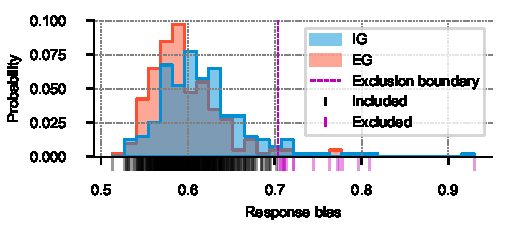
\includegraphics[width=.75\columnwidth]{Figures/c4/fig_s1.pdf}
    \caption[short Appendix figure description]{Distribution of response bias scores ($N=400$) used to exclude participants who were disengaged in performing the task. Vertical bars underneath the plot show individual data-points. The exclusion criterion, depicted as a vertical dashed line, was set to 2 standard deviations. Source data are provided as a Source Data file.}
    \label{fig:CH4A_1_exclusion_criteria}
\end{figure}

We excluded 15 participants (11 in \ac{EG} and 4 in \ac{IG} group) based on a response bias criterion that characterized the level of engagement in the task. Response bias was defined as:

\begin{equation}
    \textrm{response bias} = \frac{1}{K} \sum_{k=1}^{K}\max(p_k, 1-p_k)
\end{equation}
where $K = 4$ is the number of learning activities and $max(p_k, 1-p_k)$ denotes the relative frequency of the more frequently chosen response category in activity k. It corresponds to the participant’s tendency to choose one kind of response across all trials.

\cref{fig:CH4A_1_exclusion_criteria} shows the joint distribution of response bias scores in our sample, grouped by instruction. The figure also shows the excluded participants and the exclusion criterion. The vast majority of participants were below 0.7 which corresponded to 2 standard deviations above the mean. Relative to the included participants, the excluded ones had significantly shorter reaction times to choose a category (M = 1023.89, SD = 720.770 vs M = 1472.44, SD = 360.020; $t(23.99) = -4.484,\ p < .01$, Welch two-sample test) and significantly lower difficulty-weighted final percent-correct scores (\ac{dwfPC}; M = .689, SD = .090 vs M = .704, SD = .080; Welch two-sample test, $t(19.93) = -2.361,\ p = .029$), suggesting that they responded in a stereotyped fashion without being engaged in the task.

\begin{table*}[bh!]
    \centering
    \caption[short Appendix figure description]{Results of quadratic-regression fits of average SC on activity preference for each pairwise preference of a harder over easier activity. Source data are provided as a Source Data file.}
    \label{tab:S4}
    \begin{tabular}{ccccc}
    \hline
    \multicolumn{1}{l}{}     & \multicolumn{1}{l}{} & coef   & \textit{$t$} & \textit{$p$} \\ \hline
    \multirow{3}{*}{A2 - A1} & intercept            & 0.452  & 69.079       & $< .01$      \\
                             & pref                 & 0.033  & 5.636        & $< .01$      \\
                             & pref$^2$             & -0.060 & -17.615      & $< .01$      \\ \hline
    \multirow{3}{*}{A3 - A1} & intercept            & 0.426  & 59.860       & $< .01$      \\
                             & pref                 & 0.078  & 12.060       & $< .01$      \\
                             & pref$^2$             & -0.034 & -8.470       & $< .01$      \\ \hline
    \multirow{3}{*}{A3 - A2} & intercept            & 0.408  & 48.276       & $< .01$      \\
                             & pref                 & 0.048  & 6.163        & $< .01$      \\
                             & pref$^2$             & -0.016 & -4.383       & $< .01$      \\ \hline
    \multirow{3}{*}{A4 - A1} & intercept            & 0.397  & 62.827       & $< .01$      \\
                             & pref                 & 0.126  & 23.322       & $<.01$       \\
                             & pref$^2$             & -0.004 & -1.096       & $= .274$      \\ \hline
    \multirow{3}{*}{A4 - A2} & intercept            & 0.383  & 50.161       & $< .01$      \\
                             & pref                 & 0.100  & 14.971       & $< .01$      \\
                             & pref$^2$             & 0.009  & 2.373        & $= .019$      \\ \hline
    \multirow{3}{*}{A4 - A3} & intercept            & 0.372  & 44.348       & $< .01$      \\
                             & pref                 & 0.058  & 7.736        & $< .01$      \\
                             & pref$^2$             & 0.02   & 5.232        & $< .01$      \\ \hline
    \multicolumn{5}{l}{Note: $t$-tests compare coefficient values against 0 (df = 362)}     
    \end{tabular}
\end{table*}


\section{Self-Reported Ratings}\label{CH4A_S_self_reported_ratings}

\begin{figure}[tbh]
    \centering
    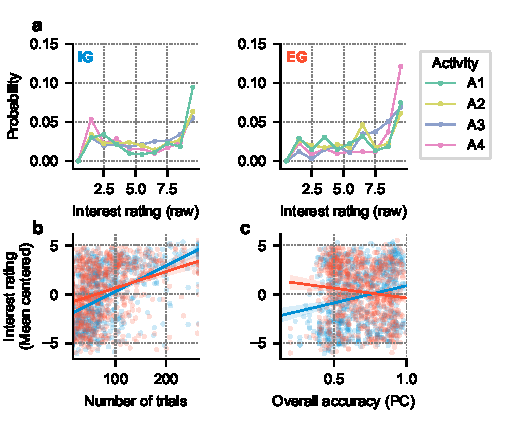
\includegraphics[width=.75\columnwidth]{Figures/c4/fig_s2.pdf}
    \caption[]{\textbf{a}, Histograms of the raw retrospective interest ratings (1 to 10; collected after the free-play stage) for each activity in the \ac{IG} (left; $N=186$) and \ac{EG} (right; $N=196$) groups show that both groups had modes for the highest rating (10). \textbf{b}, Relationship between self-reported interest ($y$-axis) and number of trials for which an activity was chosen ($x$-axis). \textbf{c}, Relationship between self-reported interest ($y$-axis) and overall activity accuracy ($x$-axis). Note, in \textbf{b} and \textbf{c}, raw data points are presented for each instruction group (red for \ac{EG} and blue for \ac{IG}); regression lines are fitted separately for each group; error bands correspond to 95\% confidence intervals for the linear predictions. Source data are provided as a Source Data file.}
    \label{fig:CH4A_2_self_reported_ratings}
\end{figure}

We collected self-reported ratings about all 4 activities at two different points of the task. Immediately after the familiarization stage (see Methods in the main article), participants were asked to report a single judgment of prospective learnability for each task: 

\begin{itemize}
\item \textit{Prospective learnability}: Before continuing, please rate each monster family based on how much you think you can learn about its food preferences during the rest of the task ([1] Definitely cannot learn more -- [10] Definitely can learn more)
\end{itemize}

After responding to the first post-familiarization question, participants proceeded to play out the free-choice stage, after which we collected 6 additional ratings: 

\begin{itemize}
\item \textit{Interest}: Rate each monster family based on how much you were interested in discovering what they preferred eating ([1] Less interested -- [10] More interested)
\item \textit{Complexity}: Rate each monster family based on how complex you thought they were ([1] Less complex -- [10] More complex)
\item \textit{Rule}: Rate each monster family based on how likely you think it had a rule for food preferences ([1] Definitely no rule -- [10] Definitely a rule)
\item \textit{Potential future learning}: Rate each monster family based on how much more you think you could learn if you had more time to play with it ([1] Definitely could not learn more -- [10] Definitely could learn more)
\item \textit{Time spent}: Rate each monster family based on how much time you spent on them ([1] Less time -- [10] More time)
\item \textit{Progress made}: Rate each monster family based on how much progress you felt you made for learning their food preferences ([1] Less progress -- [10] More progress)
\end{itemize}

The subjective reports enabled us to assess how participants felt about various aspects of our task. Specifically, we were interested in two questions: and (2) 

\begin{itemize}
    \item How well did participants track their performance and choices during free exploration? Analyses of the progress ratings showed that participants had some awareness of their performance in both the \ac{EG} and \ac{IG} groups. Across participants and activities, self-reported Progress made was significantly correlated with true progress made (the difference between \ac{PC} on the last 15 and first 15 trials on each activity; \ac{EG}: $r(750)= .286, \ p < .001$; \ac{IG}: $r(706)= .427, \ p < .001$). Similarly, self-reported Time spent was highly correlated with the true number of trials played (Pearson correlations, \ac{EG}: $r(750)= .336,\ p < .001$; \ac{IG}: $r(706)= .476,\ p < .001$). Thus, participants in both \ac{EG} and \ac{IG} groups accurately evaluated the relative time allocation and the progress they made across learning activities.
    \item How interested were they in the activities? Although participants dutifully completed the requested 250 trials of the task, they could have, in principle, reported that they were not at all interested in the activities. Contrary to this view, the distribution of Interest ratings showed a strong peak at the highest rating (10) and the average ratings were above 5 even for the activities with the lowest average ratings in each group (A4 in \ac{IG}: M = 5.371, SD = 3.432, and A1 in \ac{EG}: M = 5.934, SD = 3.118; \cref{fig:CH4A_2_self_reported_ratings}, \textbf{a}). Importantly, interest ratings scaled with the number of trials spent on each activity above and beyond the success rates (\cref{fig:CH4A_2_self_reported_ratings}, \textbf{b}). A linear regression model of mean-centered interest rating as a function of the total time spent on an activity (controlling for overall accuracy (\ac{PC} over 250 trials) and the instruction received, \ac{IG} vs \ac{EG}), showed that ratings were reliably predicted by the actual time spent in both the \ac{IG} and \ac{EG} groups (slope for \ac{IG} group = 7.966, $t(1454) = 15.204,\ p < .001$; interaction slope = -2.941, $t(1454) = -3.957,\ p < 0.001$).  Importantly, this relation was independent of any effect of \ac{PC}, suggesting that interest reflected more than mere success rates. Moreover, the correlation between \ac{PC} and interest ratings was not significant in the \ac{IG} group (slope = 0.379, $t(1454) = 0.646,\ p = .518$; \cref{fig:CH4A_2_self_reported_ratings}, \textbf{b}), and negative in the \ac{EG} group (interaction slope = -2.941, $t(1454) = -3.957,\ p < .001$; \cref{fig:CH4A_2_self_reported_ratings}, \textbf{b}), suggesting that participants had an interest in the task that was above and beyond maximizing correct feedback.
\end{itemize}

\section{Mastery Points}\label{CH4A_S_mastery_points} 

\begin{figure}[tbh]
    \centering
    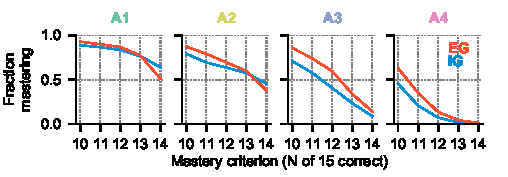
\includegraphics[width=.75\columnwidth]{Figures/c4/fig_s3.pdf}
    \caption[short Appendix figure description]{Fractions of participants mastering each activity as a function of mastery criterion and group. Changing the criterion does not change the relative proportions of participants mastering each activity.}
    \label{fig:CH4A_3_mastery_points}
\end{figure}


The learning criterion we present in the main text was based on people achieving 13 of 15 consecutive correct trials on an activity, which is equivalent to \ac{PC} = 86.7\% (probability $p = 0.0037$ of occurring by chance, assuming a binomial distribution with $n=15$). To ensure that our conclusions were robust to choice of criterion, we repeated the analyses with criteria of 10, 11, 12, 13, and 14 correct trials out of 15. As expected, the fraction of people mastering each task declined as the criterion increased but, critically, the relative frequencies of the NAM designations between \ac{EG} and \ac{IG} groups do not change (\cref{fig:CH4A_3_mastery_points}). To test this, we performed a logistic regression of reaching the criterion (0 or 1) as a function of criterion and group (\ac{EG}/\ac{IG}). We performed a separate regression for each learning activity. We used repeated contrasts for the criterion factor to compare the fractions of participants mastering a task between the adjacent levels of the factor (i.e., comparing 10 vs 11, 11 vs 12, and so on), and regular treatment contrasts to compare fractions between groups. 

The regressions produced no significant interactions between group and criterion (all $p > .05$) with only one exception: the mastery criterion of 14/15 correct was significantly less likely to be reached compared to 13/15 in the \ac{IG} group (slope = -1.035, $Z(1909) = -4.155,\ p < .001$) and even less likely in the \ac{EG} group (interaction slope = -0.802, $Z(1909) = -2.252,\ p < .024$). These results show that the differences between instruction groups were mostly stable over a range of criteria (as shown in \cref{fig:CH4A_3_mastery_points}). The positive result for the 14/15 vs 13/15 contrast shows that exceptionally high performance (\ac{PC} = 94\%) was more likely to be reached on the easiest task and that \ac{EG} participants seemed less interested in reaching this level of accuracy. Despite this effect, these mostly nonsignificant results show that an important observation holds across a range of mastery criteria: a significant fraction of the \ac{IG} group achieved mastery without being instructed to maximize learning.


\section{The Self-Challenge Index}\label{CH4A_S_self_challenge_index} 

\begin{figure}[bh!]
    \centering
    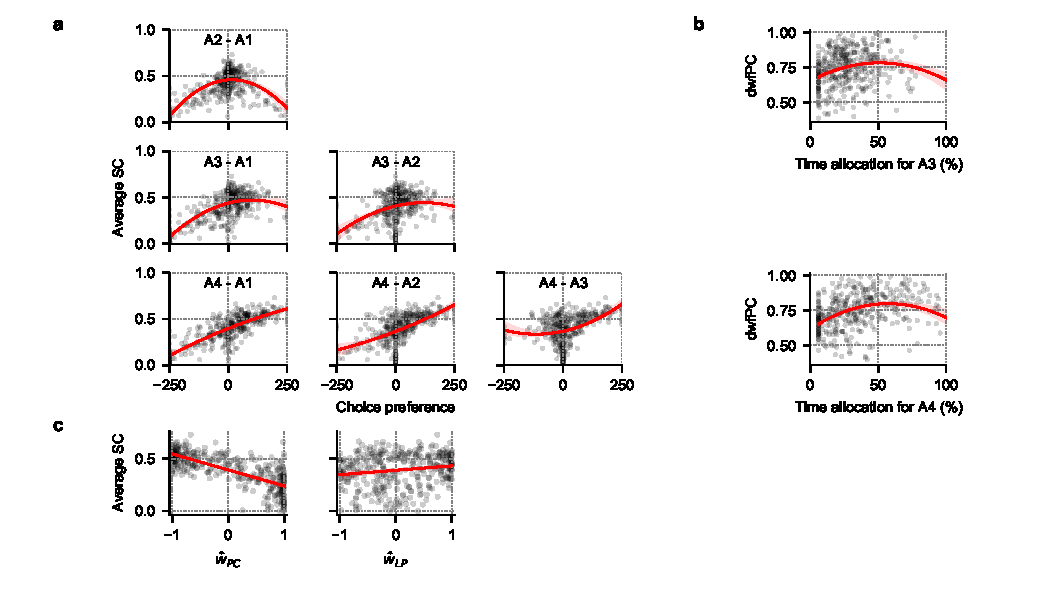
\includegraphics[width=1.1\textwidth]{Figures/c4/fig_s4.pdf}
    \caption[short Appendix figure description]{\textbf{a}, Correlation between behavioral preferences for harder activities ($x$-axes) and average SC ($y$-axis). Each point indicates one participant (pooled across groups: \ac{EG}, $N=188$ and \ac{IG}, $N=177$). In each panel, the $x$-axis is constructed so that positive values show preference for the more difficult of the two contrasted activities. \textbf{b}, Correlation between time allocation scores ($x$-axis) and difficulty-weighted final performance (\ac{dwfPC}; y-axis). \textbf{c}, Correlations between the normalized fitted coefficients ($x$-axes) and average SC ($y$-axis). In all the panels, red lines show fits of linear-quadratic regressions with error-bands (shaded regions) indicating 95\% confidence intervals (details for the fits in \textbf{a} are provided in \cref{tab:S4}). Source data are provided as a Source Data file.}
    \label{fig:CH4A_4_self_challenge_index}
\end{figure}

We conducted several analyses that established that our SC measure captured the tendency to choose more difficult activities (\cref{fig:CH4A_4_self_challenge_index}, \textbf{a}), did not bias our conclusions (\cref{fig:CH4A_4_self_challenge_index}, \textbf{a}), and showed the expected correlations with the model coefficients (\cref{fig:CH4A_4_self_challenge_index}, \textbf{c}).

As shown in \cref{fig:CH4A_4_self_challenge_index} (\textbf{a}), the SC index showed a positive correlation with all possible pairwise measures of the preference for the harder activities, confirming that it measured self-challenge. However, several of these relationships were non-linear, indicating that pairwise differences do not fully capture the choices in our 4-alternative task (see \cref{tab:S4} for full details on the regression fits). Specifically, the preferences for activities with moderate difficulty (A2 or A3) had an inverted U-shape trend indicating that, if these preferences were too strong, they implied lower SC by virtue of withdrawal from the most difficult activity. Similarly, the contrast of A4 vs A3 showed an upright U-shaped profile, indicating that a lower preference for A4 can correspond with higher SC if people strongly prefer A3 over A1 and A2. Thus, in our 4-alternative choice experiment, the SC index is a more parsimonious measure of the preference for challenging tasks relative to measures of preference between specific pairs of tasks.

As additional confirmation, we verified that the inverted-U relationships between SC and \ac{dwfPC} shown in the main text (4) was replicated if we replaced SC with the preference for A3 or A4 (\cref{fig:CH4A_4_self_challenge_index}, \textbf{b}). In case of A3’s time allocation, the linear-quadratic model was better than its non-quadratic counterpart ($\Delta \mathrm{AIC} = 22.238$) and showcased a significant negative coefficient for the quadratic term (slope = -0.016, $t(361) = -4.979,\ p <.001$). A similar linear-quadratic model featuring time allocation for activity A4 was also better than the corresponding non-quadratic model ($\Delta \mathrm{AIC} = 26.178$) and likewise had a significant coefficient for its quadratic term (slope = -0.026, $t(361) = -5.383,\ p < .001$). Together, the results from \cref{fig:CH4A_4_self_challenge_index}, (\textbf{a}, \textbf{b}), demonstrate that SC served as a parsimonious measure of activity preferences and did not bias the results we report.

Finally, we examined how SC was related to the fitted (bivariate) computational-model coefficients (\cref{fig:CH4A_4_self_challenge_index}, \textbf{c}). SC was negatively correlated with $w_\mathrm{PC}$ (slope = -0.153, $t(361) = -21.999,\ p < .001$), consistent with our intuitions that choosing activities with lower \ac{PC} corresponds to self-challenging choices. The regression also showed a positive correlation with $w_\mathrm{LP}$ (slope = 0.042, $t(361) = 4.954,\ p < .001$), consistent with the prediction that a sensitivity to \ac{LP} guides learners to venture beyond what’s easy and familiar, and choose moderately challenging activities.


\section{Individual Model Fit: A Case Study}\label{CH4A_S_individual_model_fit}

\begin{figure}[bh!]
    \centering
    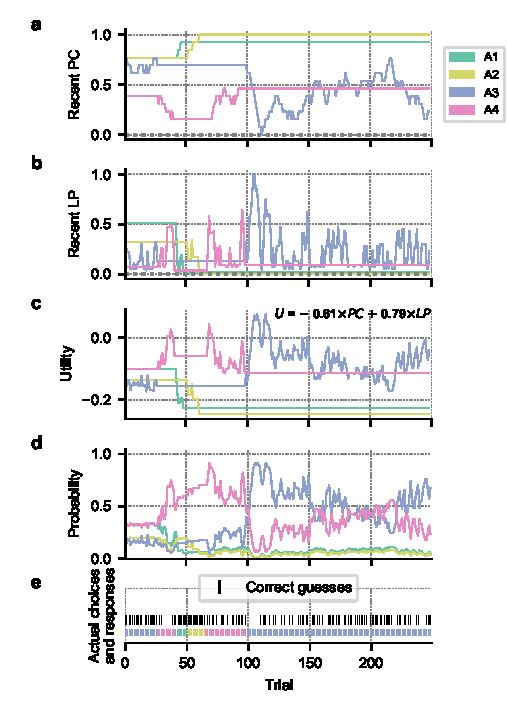
\includegraphics[width=.75\columnwidth]{Figures/c4/fig_s5.pdf}
    \caption[short Appendix figure description]{The $x$-axis shows 250 trials of free play. Each of the first four subfigures shows the choice features of each activity through time. \textbf{a}, normalized recent percent correct (PC); b, normalized recent learning progress (LP); \textbf{c}, utility computed as a linear combination of \ac{PC} and \ac{LP}. The utility equation shows coefficients normalized by the Euclidean norm of the $w_{\mathrm{PC}}$ and $w_{\mathrm{LP}}$ coefficients; \textbf{d}, choice probabilities given by a softmax function at the fitted temperature parameter, $\tau = 84.98$; \textbf{e}, empirical data that the model was fitted to. The colored bar represents the observed sequences of activity choices (A3$\rightarrow$A4$\rightarrow$A1$\rightarrow$A2$\rightarrow$A4$\rightarrow$A3) and the black vertical sticks show correct responses. Source data are provided as a Source Data file.}
    \label{fig:CH4A_5_individual_model_fit}
\end{figure}

\cref{fig:CH4A_5_individual_model_fit} demonstrates our model fitting procedure and model-based simulations for one participant’s data. Panels \textbf{a} and \textbf{b} show, respectively, the participant’s values of \acf{PC} and \acf{LP} values over time. \ac{PC} and \ac{LP} remained constant if the participant did not choose a task, explaining the long horizontal lines on the plots. Panel \textbf{c} shows the dynamic utility for each task based on the participant’s fitted coefficients (given in the equation). Panel \textbf{d} shows the probabilities of choosing each task, simulated using the corresponding utility and the softmax function with the best-fit temperature parameter. 

In this particular model, the participant’s choices were characterized by a preference towards activities with high \ac{LP} and low \ac{PC}, which results in a model that predicted high probabilities of choosing A3 and A4 activities. Activities A1 and A2, which had consistently high \ac{PC} values generated low utility and were infrequently chosen. This model captures well the transition from A4 to A3 around trial 100, where the utility of A4 started dropping as a result of a low \ac{LP} signal and a corresponding plateauing of the \ac{PC} signal (\cref{fig:CH4A_5_individual_model_fit}, \textbf{a}, \textbf{b}, and \textbf{d}).

\section{Familiarity Component}\label{CH4A_S_familiarity_component}

\begin{figure}[t!]
    \centering
    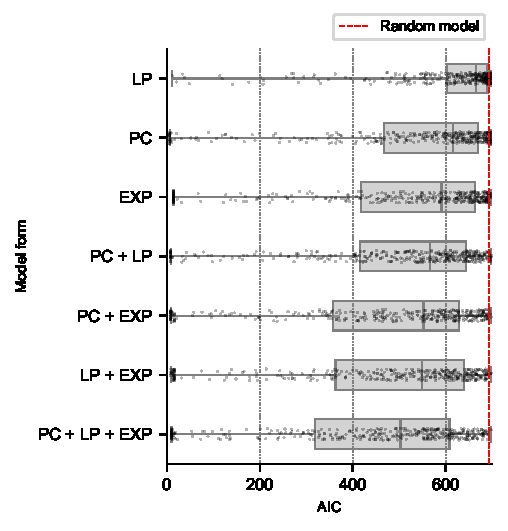
\includegraphics[width=.75\columnwidth]{Figures/c4/fig_s6.pdf}
    \caption[short Appendix figure description]{Distributions of AIC scores for all model subsets of the full trivariate model \ac{PC} + \ac{LP} + \ac{EXP}, where \ac{EXP} represents count-based task familiarity. The box-plot box boundaries represent the 1st and the 3rd quartiles; middle bars represent sample medians; whiskers show sample minima and maxima. The random (baseline) model has AIC = 693.147 and no variance. Individual data points ($N=365$ per model form) are shown in the overlaid strip-plots. Source data are provided as a Source Data file.}
    \label{fig:CH4A_6_familiarity_component}
\end{figure}

The model comparisons from the main text show that on average, the bivariate utility function (\ac{PC} + \ac{LP}) explains participant’s choices better than the univariate models. The measures of \ac{PC} and \ac{LP} capture different aspects of competence that were hypothesized to function as intrinsic reward signals for a freely exploring learner. Different analogs of these measures have been widely used in the computational literature on intrinsically motivated learning, e.g., \parencite{colas_curious_2019,bougie_skill-based_2019}. These measures can be characterized as competence-based measures, because they track the information about one’s competence in performing a task. There are other important families of approaches which we did not include in our study. For instance, we did not include any predictive knowledge-based measures, which would require to explicitly model the participants’ beliefs about food preferences. This is an interesting direction for future work, but these kinds of models entail considerable additional complexity that is outside the scope of our investigation. However, we could test another kind of knowledge-based curiosity measure, which does not require an internal predictive model. In computational literature, this approach is referred to as a count-based, because it relies on state visitation counts \parencite{bellemare_unifying_2016}. State visitation counts can be interpreted as state familiarity (the opposite of novelty).

Due to the reasoning laid out below, we did not include the measure of familiarity in the main report of model comparisons, even though it is a central idea behind some approaches to intrinsically motivated exploration. The rationale for omitting this component from the reported analyses was our focus on the roles of learning-based heuristics in the self-determined selective engagement in one of several learning activities. The familiarity measure, as defined below, is based directly on the participant’s choices and as such is completely orthogonal to the dynamics of a learner’s competence. Since a single episodic sampling of a learning activity contributes to the measured familiarity of all activities equally, familiarity measured this way does not merely correlate with activity choices, it is completely determined by them. Such a measure of familiarity is a good predictor of the choice of activity, but it does not explain the choice very well. Thus, even if familiarity was an important component for the utility-based prediction (which is indeed the case), it would not be a good explanatory variable, because it itself is determined by choices.

Here we discuss a more extensive model comparisons exercise which included the additional familiarity component on top of those reported in the main text. We operationalized familiarity as exposure (\ac{EXP}) to a learning activity, defined as a min-max normalized count of choice of activity. Specifically, we simply counted the number of times an activity was chosen by a participant on each trial of free play, and then re-scaled the counts to be between 0 and 1, using min-max normalization (this normalization was also applied to all \ac{PC} and \ac{LP} before fitting the models): 

\begin{equation}
    \mathrm{norm}(\mathrm{count}_{t,i}) = \frac{\mathrm{count}_{t,i} - \min(\mathrm{counts})}{\max (\mathrm{counts}) - \min (\mathrm{counts})}
\end{equation}

Where $\mathrm{count}_{t,i}$ is the number of times on which activity $i$ was selected prior to trial $t$, and $\max(counts)$ and $\min(counts)$ denote, respectively, the maximum and minimum counts across all tasks and trials.

The \ac{EXP} measure was added to the set of potential utility function components for all-subsets model comparisons. Fig \cref{fig:CH4A_6_familiarity_component}. presents the distributions of AIC scores of each subset of variables included in the model. The full-form trivariate model (\ac{EXP} + \ac{PC} + \ac{LP}) had the lowest AIC on average (M = 438.068, SD = 212.092). Thus, even when familiarity was included in the mix, both \ac{PC} and \ac{LP} were still important factors in increasing model likelihood. These results further support the importance of learning-based heuristics for the self-determined choice of activity. At the individual level, when compared to all of the other 6 model forms, the trivariate model (\ac{EXP} + \ac{PC} + \ac{LP}) had the lowest AIC score in only 49.59\% of participants (\cref{fig:CH4A_4_self_challenge_index}) and was at least 2 points less than any other model in only 38.90\% of individuals. Moreover, the median AIC scores of the trivariate model and the next best fitting model among individuals was nonsignificant ($Z(365) = 181,\ p = .917$). These results show that although the \ac{EXP} component provided some further improvement in likelihood over other models, this improvement was not very substantial: the \ac{PC} + \ac{LP} bivariate were, on average, significantly better than univariate models, as reported in the main text.

On the other hand, models that included both \ac{PC} and \ac{LP} components (i.e., \ac{EXP} + \ac{PC} + \ac{LP} and \ac{PC} + \ac{LP}) had the lowest AIC in 73.42\% of cases. Furthermore, compared to any univariate model -- including the \ac{EXP}-only model -- the bivariate (\ac{PC} + \ac{LP}) model showed reliably better AIC scores ($Z(365) = 365,\ p = .021$, Wilcoxon signed-rank test). Notwithstanding the predictive power of the \ac{EXP} component alone, \ac{PC} and \ac{LP} components remain important predictors of self-determined activity choices.


\section{Model Coefficients and Activity Preferences}\label{CH4A_S_model_coefficients}

\begin{figure}[th]
    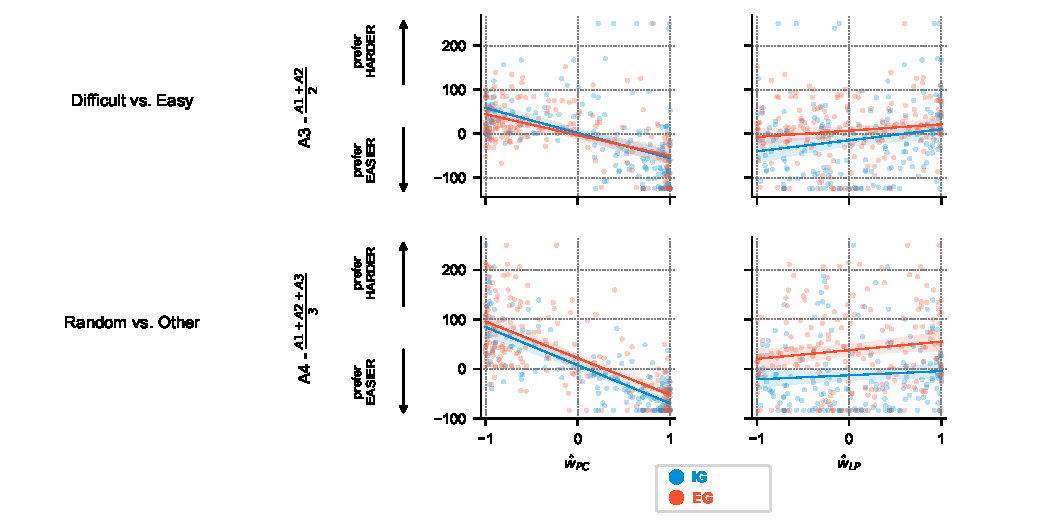
\includegraphics[width=1.1\textwidth]{Figures/c4/fig_s7.pdf}
    \caption[short Appendix figure description]{Each point is one participant in the \ac{IG} (blue, $N=177$) and \ac{EG} (red, $N=188$) group. The $y$-axis shows the difference between the number of trials a participant chose A3 minus the average number of trials spent on A1 and A2; the bottom row compares the random activity to all other activities. The $x$-axis shows the normalized $w_{\mathrm{PC}}$ and $w_{\mathrm{LP}}$ coefficients from the bivariate models. The lines represent linear models of activity difficulty preference as a function of normalized coefficients (each line pair fitted separately for the corresponding subplot; shaded regions represent 95\% confidence intervals). $w_{\mathrm{PC}}$ coefficients (negative values indicating the tolerance for errors) were associated with choices of harder activities regardless of their learnability (left column). In contrast, $w_{\mathrm{LP}}$ coefficients (indicating more sensitivity to performance derivatives) were positively related to a preference for a harder activity only when that activity was learnable (top right), but not when it was unlearnable (bottom right). Source data are provided as a Source Data file.}
    \label{fig:CH4A_7_model_coefficients}
\end{figure}

As we discuss in the main text, \ac{PC} and \ac{LP} may play distinct roles in self-regulated learning. While \ac{PC} can help learners identify challenging activities, \ac{LP} can be used to avoid unlearnable activities. To examine this idea further, we analyzed how the $w_\mathrm{PC}$ and $w_\mathrm{LP}$ coefficients (normalized to reflect relative preferences as explained in the text) correlated with individual preferences for challenging over easier activities when the more challenging activity was, respectively, learnable or unlearnable. As a simple measure of the tendency to choose more challenging learnable activities, we computed the difference between the number of trials a participant devoted to activity A3 relative to the average amount of trials spent on easier activities (A1 and A2, \cref{fig:CH4A_7_model_coefficients}, top row). As a measure of the tendency to choose the more challenging random activity, we computed the difference between the number of trials devoted to activity A4 relative to the average amount of time spent on other activities (A1, A2, and A3; \cref{fig:CH4A_7_model_coefficients}, bottom row). 
        
The $w_\mathrm{PC}$ coefficients showed negative correlations with both measures, suggesting that they captured the participants’ tendency to choose more difficult tasks regardless of learnability (\cref{fig:CH4A_7_model_coefficients}, left). Both the preference for A3 and the preference for A4 showed negative correlations with $w_\mathrm{PC}$ (A3 vs A1\&A2; \ac{IG} slope = 56.969, $t(361) = -8.255,\ p < .001$; A4 vs A1-A3 slope = 86.684, $t(361) = -13.822,\ p < .001$).

In contrast, in the \ac{IG} group, the $w_\mathrm{LP}$ coefficients showed a positive relationship with the preference for A3 (slope = 25.060, $t(361) = 2.817,\ p = .006$), but no relationship with the preference for A4 ($p = .356$; \cref{fig:CH4A_7_model_coefficients}, right), suggesting that people with higher $w_\mathrm{LP}$ coefficients tended to prefer the more difficult activity only if that activity was learnable. The \ac{EG} group showed no significant relationship between $w_\mathrm{LP}$ coefficients and either measure of preference. 
        
Given the predictions of the \ac{LP} hypothesis, one might expect to actually find a negative relationship between \ac{LP} and a preference for an unlearnable task, not just a lack of a relationship. Indeed, one of the appeals of the \ac{LP} heuristic is that it protects the learner from fixating on low-performance activities when it is not worth it. While we did not find evidence strongly supporting or refuting this prediction, we identify two ways in which it can be obtained. First, it is possible that our rather restricted operationalization of \ac{LP} was not optimal for differentiating between activities A3 and A4, which were indeed very similar in terms of their recent-feedback patterns. The \ac{LP} signal was especially noisy compared to the relatively clear \ac{PC} signal. Investigating a wider scope of models with alternative formulations of \ac{LP} could be useful for testing the predicted preference for learnable vs unlearnable tasks. Another approach would be to implement an experimental setting similar to ours, but with a larger amount of difficult learnable and unlearnable tasks. Such a setting would be more effective in showing whether sensitivity to \ac{LP} helps to avoid activities that are impossible to learn.

\end{subappendices}